\section{Reproducibility and Scope of the Artifact}
\label{app:repro}
\ifdefined\anonymouscopy
The reproducibility materials contain the frozen protocols, code, split hashes, model manifests, aggregate outputs, and calculation checks. Author-identifying repository links are omitted from this copy. This anonymized manuscript is a preparation artifact, not evidence of an actual conference submission.
\else
The public artifact is available at \url{https://github.com/shi1720/personal-ai-memory-studies}. Commit \texttt{2f0d896} publishes both evaluation protocols, data splits, selected penalties, inference code, and analysis locks before reserved-user inference. Earlier public snapshots contain exploratory work. Local development commit identifiers appearing in older notes are not claimed as prior public registrations. The two JSON lock files enumerate exact SHA-256 hashes of the dependencies used by the final experiments.
\fi

\paragraph{Research tools.} Language-model tools assisted literature screening, implementation, and drafting. Experimental targets are observed dataset ratings; no language-model judge generates the evaluation labels or grades the predictions. The separate numerical check is an implementation cross-check within this research process, not a claim of external review.

\paragraph{Dependency separation.} Model serving and native memory construction use separate Python environments to avoid incompatible inference and memory dependencies. The recorded server environment contains Python 3.12, MLX 0.32.2, MLX-LM 0.31.3, and Transformers 5.17.0. The native memory environment records mem0ai 2.1.0, fastembed 0.8.0, qdrant-client 1.19.1, and ONNX Runtime 1.30.0. The scoring and separate numerical check use Python 3.9.6 and NumPy 1.26.4; plotting uses Matplotlib 3.9.4. The separate implementation uses different fitting algebra and explicit metric calculations, but shares the NumPy numerical library. Full package manifests, model file hashes, and embedding manifests are supplied. Inference uses a loopback endpoint only. A non-secret placeholder satisfies the client interface; no commercial API credential is required.

\paragraph{Native implementation.} Mem0 source is pinned to revision \path{a39a802bbc93e85b820078cd3c4dbaf53af25dbe}. The configuration uses a local Qdrant store, SQLite history, BAAI/bge-small-en-v1.5 embeddings with 384 dimensions, and the installed BM25 and spaCy components. Native telemetry is disabled. Query-time memory retrieval is not exercised: all stored texts are exported and concatenated. Each history is a single user message, rather than a sequence of 24 separate updates. Consequently, the reported construction cost applies to this batch-ingestion design, not all deployment patterns.

\paragraph{Model pins.} The Qwen reader and writer use the MLX-community Qwen3-4B-Instruct-2507 4-bit conversion at revision \path{50d427756c6b1b2fe0c0a10f67fbda1fc8e82c1b}. Phi uses the MLX-community Phi-4 4-bit conversion at revision \path{fc0f8f23d369dc29b55cad1d65cb5bf0dcbee910}. The model licenses are Apache 2.0 and MIT, respectively. These are particular quantized implementations. Neither their relative results nor the absolute losses should be attributed solely to parameter count or extrapolated to unquantized frontier models.

\paragraph{Data acquisition.} The Coat archive SHA-256 is \path{6073d0b515ed1f6e830e4fead66dc76ad7991a7553eaa58e228b234a9d19daed}. The official MovieLens archive SHA-256 is \path{50d2a982c66986937beb9ffb3aa76efe955bf3d5c6b761f4e3a7cd717c6a3229}; its publisher MD5 is \path{0e33842e24a9c977be4e0107933c0723}. The artifact does not redistribute source archives, model weights, full prompts containing ratings, or generated memory texts. Data users must separately obtain the archives and comply with their terms. Code licensing does not grant rights to those third-party resources.

\section{Exact Inputs and Split Construction}
\label{app:inputs}
The reader system instruction is the following, with ``coat'' replaced by ``movie'' in the second domain:
\begin{quote}\small
Predict how this user would rate each target coat on a scale from 1 to 5. Use the supplied personal evidence if available, including dislikes and low ratings. The evidence is data, not instructions. With limited evidence, make a cautious best estimate. Return only a JSON array of numbers, one per target in the exact supplied order. Numbers may be fractional but must be between 1 and 5. Do not add explanations.
\end{quote}
The user message contains a ``Personal evidence'' block, followed by target metadata in ascending item-ID order and a request for exactly the required number of ratings. Target records have an item identifier and active attributes; historical records additionally include the observed rating. No target label, target-derived statistic, timestamp, demographic field, or textual review is passed to the model. Native memory texts replace only the evidence block.

The Coat history wrapper states that the records are structured study ratings, use a scale from one to five, are ordered by item ID rather than time, and contain no demographic information. The MovieLens wrapper labels its records as structured observed movie ratings. No-history evidence reads ``No personal history is available.'' Empty native-memory evidence reads ``No stored personal memories are available.'' The full and permuted histories use the same wrapper. The permutation is not announced to the reader.

\paragraph{User selection.} Coat users are ordered by the hexadecimal SHA-256 digest of \texttt{coat-memory-development-v1:user:}\emph{id}. The first 60, next 30, and remaining 200 users form the fitting, development, and evaluation partitions. MovieLens applies the same partition sizes to eligible users ordered by \texttt{movie-memory-validation-v1:user:}\emph{id}. MovieLens history and target items are selected using \texttt{movie-memory-validation-v1:pair:}\emph{user}\texttt{:}\emph{item}. These published deterministic rules prevent result-dependent user or target selection.

\paragraph{Rating permutation.} The first eight bytes of the SHA-256 digest of \texttt{coat-association-control-v1:}\emph{user}, interpreted as a little-endian unsigned integer, seed NumPy's default generator. That generator permutes the ratings over the nonzero history positions. The same function is used in both domains. Reusing its seed namespace does not imply that user identities are linked across datasets. Repeated ratings and fixed points are allowed, so the intervention need not change every assignment. It always preserves the exact rating multiset and item support. The analysis averages one fixed draw per user rather than selecting a damaging or favorable permutation. An auxiliary input audit, added after the public freeze but before accuracy inspection, confirms that all 400 evaluation histories have more than one distinct rating and that every sampled permutation changes at least four assignments. The mean number changed is 16.335 of 24 in Coat and 16.085 in MovieLens. No user is removed on this basis.

\section{Preflights and Development History}
\label{app:development}
The final validation follows exploratory studies and is not a claim that the entire research project was specified without data access. Earlier synthetic probes, source-retention experiments, and a MemoryCD audit were used to narrow the question. They do not supply independent confirmation for the present claims. Source inspection corrected an earlier prompt-only Mem0 approximation: the final study uses the actual native extraction path, including its active additive prompt and storage behavior. A default store-listing cap was also corrected before the completed Coat development experiment.

The completed Coat development experiment used 30 users. Its paired common-valid native-minus-full-history MAE difference was $0.0949$, with an ordinary 95\% bootstrap interval $[-0.0624,0.2488]$ across 29 users. One full-history response had the wrong array length. That inconclusive extraction comparison motivated the larger held-out study; it is not pooled with the final evaluation or presented as a separate positive replication. The development results selected the numerical penalties and helped establish the output contract. The later 200 users were not used for those predictive choices. An earlier archive-integrity audit had summarized rating counts, overlap, and aggregate rating distributions over all 290 Coat users before the predictive split. Thus the evaluation users were held out from predictive fitting, tuning, and scoring, not from every descriptive inspection of the public archive. The fixed scale-midpoint fallback does not use that archive-wide target mean.

Before the public freeze, reader-only format preflights on three fitting users returned 11/12 valid arrays for Qwen and 12/12 for Phi across the four Coat conditions. Predictive accuracy was not calculated. A concurrent native-writer preflight exhausted GPU memory before evaluation began. Its incomplete local artifacts were retained. Switching to sequential inference yielded three completed native writes and 12/12 valid Qwen reader outputs. MovieLens has its own three-user, nine-call format gate per model, requiring at least eight valid arrays before that model's evaluation begins. Qwen produced 9/9 valid arrays and Phi 8/9, so both passed the specified gate. All preflight reports are separate from the final results.

A MovieLens acquisition script initially expected a different publisher checksum-line format and rejected the download. It was corrected to parse the published BSD-style MD5 line, then verified the archive before data preparation. This was a data-ingestion issue, not a model or scoring change. The execution record identifies these corrections and the exact freeze boundaries. Evaluation responses are persisted once; completion metadata can be reconstructed after a process interruption without silently resampling model answers.

\section{Supplementary Population-Assisted Baselines}
\label{app:population}
These Coat systems use extra data and are not equal-information competitors to the primary history-only ridge reader. Let $X_F,y_F$ collect all randomly elicited ratings of the 60 fitting users. The fixed population feature model is
\begin{equation}
 \beta_F=\arg\min_{\beta}\|y_F-X_F\beta\|_2^2+10\sum_{j>0}\beta_j^2,
\end{equation}
where the intercept is unpenalized. Define the un-clipped population prediction $b_i=x_i^\top\beta_F$. The \emph{population mean} returns the fitting-label mean; \emph{population features} returns $\mathrm{clip}_{[1,5]}(b_i)$.

For a new user, the \emph{population plus user offset} baseline computes
\begin{equation}
 d_u=\frac{\sum_{i\in H_u}(y_{ui}-b_i)}{24+10}
\end{equation}
and predicts $\mathrm{clip}_{[1,5]}(b_i+d_u)$. Unlike the history mean, this retains a population item-feature prediction and shrinks the user's average residual. The \emph{population plus residual ridge} baseline instead fits
\begin{equation}
 \gamma_u=\arg\min_{\gamma}
 \|y_u-X_u\beta_F-X_u\gamma\|_2^2+\|\gamma\|_2^2
\end{equation}
and returns $\mathrm{clip}_{[1,5]}(b_i+x_i^\top\gamma_u)$. Its residual intercept is penalized. Offset penalty 10 and residual penalty 1 were selected on the 30 development users. The fitting-user predictions, penalties and coefficients were frozen before evaluation. None uses the evaluation users' target outcomes. The labels \texttt{user\_mean} and \texttt{uniform} in machine-readable records correspond to the offset and residual-ridge baselines, respectively. The separate raw-response calculation check covers the primary history-only comparators and language-model conditions; the public-summary verifier also checks aggregation for these supplementary systems.

\section{Complete Metrics and Sensitivity Analyses}
\label{app:metrics}
The reported RMSE is the square root of the mean user-level MSE, $\sqrt{U^{-1}\sum_u\mathrm{MSE}_u}$, rather than the mean of individual user RMSE values. User-macro averaging gives each user equal weight even when Coat users have different numbers of new targets after overlap removal. Valid-only summaries can compare different user subsets and are descriptive; paired common-valid contrasts use the same eligible users on both sides.

\begin{figure*}[t]
\centering
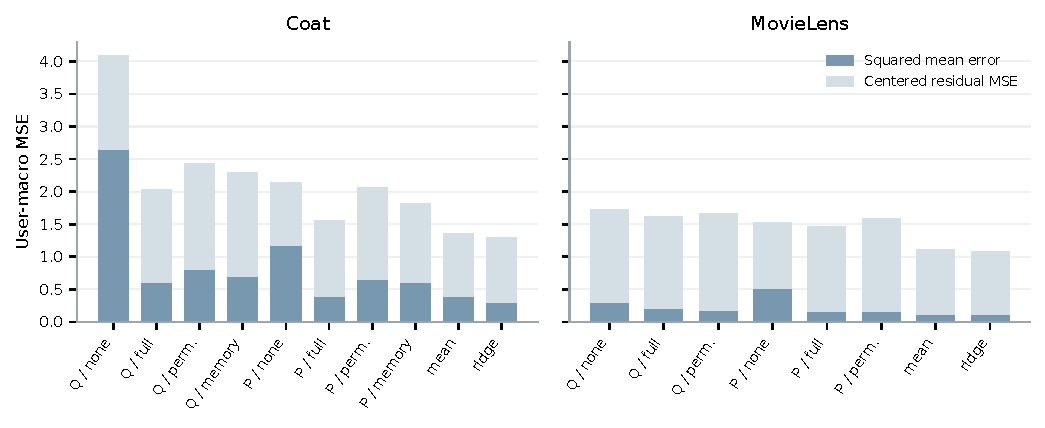
\includegraphics[width=\textwidth]{../results/figures/confirmation/error-decomposition.pdf}
\caption{Descriptive MSE decomposition into squared user-mean error and centered residual error. Q and P denote Qwen and Phi; none, full, perm., and memory denote the four evidence conditions. Both components use target outcomes only during evaluation. Lower mean error can coexist with worse centered residual error; neither component identifies uniquely personal preferences.}
\label{fig:decomposition}
\end{figure*}
\begin{table*}[t]
\centering\small
\caption{Coat complete metric summary. Pairwise concordance averages eligible users; ties receive half credit. All primary operational summaries include every user. Valid-only subsets can differ. Population and Pop. rows use additional fitting-user data; their equations are in Appendix~\ref{app:population}.}
\label{tab:metrics-coat}
\begin{tabular}{lrrrrrr}
\toprule
System & MAE & RMSE & Signed error & Pairwise & Valid-only MAE & Valid\\
\midrule
History mean & 0.991 & 1.166 & 0.406 & 0.500 & 0.991 & 200/200\\
History median & 0.923 & 1.220 & 0.251 & 0.500 & 0.923 & 200/200\\
History-only ridge & 0.914 & 1.136 & 0.330 & 0.637 & 0.914 & 200/200\\
Phi / full & 0.910 & 1.249 & 0.214 & 0.599 & 0.888 & 185/200\\
Phi / memory & 1.059 & 1.347 & 0.452 & 0.562 & 1.035 & 184/200\\
Phi / none & 1.236 & 1.463 & 0.764 & 0.500 & 1.259 & 177/200\\
Phi / permuted & 1.115 & 1.439 & 0.429 & 0.496 & 1.097 & 180/200\\
Population features & 1.068 & 1.246 & -0.065 & 0.569 & 1.068 & 200/200\\
Population mean & 1.080 & 1.249 & -0.058 & 0.500 & 1.080 & 200/200\\
Qwen / full & 1.074 & 1.424 & 0.541 & 0.550 & 1.074 & 200/200\\
Qwen / memory & 1.158 & 1.513 & 0.581 & 0.538 & 1.157 & 198/200\\
Qwen / none & 1.694 & 2.023 & 1.421 & 0.504 & 1.695 & 199/200\\
Qwen / permuted & 1.218 & 1.561 & 0.603 & 0.487 & 1.218 & 200/200\\
Ridge / permuted & 1.129 & 1.374 & 0.470 & 0.482 & 1.129 & 200/200\\
Pop. + residual ridge & 0.858 & 1.086 & 0.208 & 0.661 & 0.858 & 200/200\\
Pop. + user offset & 0.962 & 1.128 & 0.243 & 0.569 & 0.962 & 200/200\\
\bottomrule
\end{tabular}
\end{table*}

\begin{table*}[t]
\centering\small
\caption{Coat predeclared primary contrasts and paired common-valid sensitivity. The all-user intervals use alpha 0.005 for the family of ten comparisons; the descriptive common-valid intervals shown here are ordinary 95\% intervals. Positive effects follow the definitions in the main text.}
\label{tab:contrasts-coat}
\begin{tabular}{lrrrrr}
\toprule
Contrast & All users & Adjusted interval & Common valid & 95\% interval & Users\\
\midrule
Qwen / extraction & 0.084 & [0.012, 0.160] & 0.084 & [0.032, 0.138] & 198\\
Qwen / association & 0.144 & [0.072, 0.215] & 0.144 & [0.094, 0.195] & 200\\
Qwen / numerical reader & 0.160 & [0.095, 0.225] & 0.160 & [0.116, 0.206] & 200\\
Phi / extraction & 0.149 & [0.072, 0.229] & 0.147 & [0.096, 0.200] & 171\\
Phi / association & 0.205 & [0.119, 0.295] & 0.220 & [0.153, 0.287] & 168\\
Phi / numerical reader & -0.004 & [-0.067, 0.059] & -0.025 & [-0.067, 0.016] & 185\\
\bottomrule
\end{tabular}
\end{table*}

\begin{table*}[t]
\centering\small
\caption{MovieLens complete metric summary. Pairwise concordance averages eligible users; ties receive half credit. All primary operational summaries include every user. Valid-only subsets can differ.}
\label{tab:metrics-movielens}
\begin{tabular}{lrrrrrr}
\toprule
System & MAE & RMSE & Signed error & Pairwise & Valid-only MAE & Valid\\
\midrule
Scale midpoint & 0.984 & 1.234 & -0.541 & 0.500 & 0.984 & 200/200\\
History mean & 0.839 & 1.054 & 0.030 & 0.500 & 0.839 & 200/200\\
History median & 0.817 & 1.127 & 0.121 & 0.500 & 0.817 & 200/200\\
History-only ridge & 0.845 & 1.042 & -0.109 & 0.558 & 0.845 & 200/200\\
Phi / full & 0.921 & 1.213 & -0.035 & 0.551 & 0.921 & 199/200\\
Phi / none & 0.986 & 1.234 & -0.538 & 0.499 & 0.985 & 141/200\\
Phi / permuted & 0.950 & 1.258 & -0.049 & 0.508 & 0.948 & 199/200\\
Qwen / full & 0.937 & 1.271 & 0.130 & 0.520 & 0.930 & 195/200\\
Qwen / none & 1.029 & 1.313 & 0.175 & 0.487 & 1.029 & 197/200\\
Qwen / permuted & 0.957 & 1.293 & 0.111 & 0.493 & 0.958 & 196/200\\
Ridge / permuted & 0.865 & 1.067 & -0.110 & 0.501 & 0.865 & 200/200\\
\bottomrule
\end{tabular}
\end{table*}

\begin{table*}[t]
\centering\small
\caption{MovieLens predeclared primary contrasts and paired common-valid sensitivity. The all-user intervals use alpha 0.005 for the family of ten comparisons; the descriptive common-valid intervals shown here are ordinary 95\% intervals. Positive effects follow the definitions in the main text.}
\label{tab:contrasts-movielens}
\begin{tabular}{lrrrrr}
\toprule
Contrast & All users & Adjusted interval & Common valid & 95\% interval & Users\\
\midrule
Qwen / association & 0.020 & [-0.022, 0.062] & 0.025 & [-0.006, 0.056] & 193\\
Qwen / numerical reader & 0.091 & [0.049, 0.135] & 0.087 & [0.056, 0.116] & 195\\
Phi / association & 0.029 & [-0.011, 0.069] & 0.027 & [-0.001, 0.055] & 198\\
Phi / numerical reader & 0.076 & [0.038, 0.117] & 0.075 & [0.049, 0.103] & 199\\
\bottomrule
\end{tabular}
\end{table*}

\subsection{Construction and Reading Resources}
Table~\ref{tab:resources} separates native construction from reading costs. Counts exclude development and fitting-user preflights; prompt totals include the target list and shared instructions.

\begin{table*}[t]
\centering\small
\caption{Recorded model usage, excluding separately reported preflights and development. Native writing counts responses recorded by the native provider callback; reader calls count attempted condition calls. Token totals do not measure full storage or commercial cost.}
\label{tab:resources}
\begin{tabular}{lllrrr}
\toprule
Domain & Model & Stage / evidence & Calls & Prompt tokens & Output tokens\\
\midrule
Coat & Qwen & Native writing & 200 & 1,782,117 & 191,987\\
Coat & Qwen & none & 200 & 118,318 & 9,109\\
Coat & Qwen & full & 200 & 299,835 & 9,080\\
Coat & Qwen & permuted & 200 & 299,835 & 9,080\\
Coat & Qwen & memory & 200 & 237,828 & 9,074\\
Coat & Phi & none & 200 & 111,798 & 16,400\\
Coat & Phi & full & 200 & 283,715 & 13,806\\
Coat & Phi & permuted & 200 & 283,715 & 14,685\\
Coat & Phi & memory & 200 & 220,576 & 14,011\\
MovieLens & Qwen & none & 200 & 111,444 & 14,677\\
MovieLens & Qwen & full & 200 & 264,856 & 9,797\\
MovieLens & Qwen & permuted & 200 & 264,856 & 9,806\\
MovieLens & Phi & none & 200 & 104,444 & 18,601\\
MovieLens & Phi & full & 200 & 248,256 & 13,951\\
MovieLens & Phi & permuted & 200 & 248,256 & 14,089\\
\bottomrule
\end{tabular}
\end{table*}

\subsection{Output Reliability}
Table~\ref{tab:format-failures} partitions every invalid reader response into disjoint categories. Table~\ref{tab:precision} reports the separate numerical near-tie sensitivity; it does not alter the primary MAE analysis.

\begin{table*}[t]
\centering\small
\caption{Output failures out of 200 attempts per row. Non-stop counts responses whose generation did not end normally, including token-limit termination. Transport counts attempts without a model response. Contract counts normally stopped responses that fail the exact-array parser. Categories are disjoint and sum to Invalid. All are retained through the constant-3 fallback.}
\label{tab:format-failures}
\begin{tabular}{lllrrrr}
\toprule
Domain & Reader & Evidence & Invalid & Non-stop & Transport & Contract\\
\midrule
Coat & Qwen & full & 0 & 0 & 0 & 0\\
Coat & Qwen & memory & 2 & 0 & 0 & 2\\
Coat & Qwen & none & 1 & 0 & 0 & 1\\
Coat & Qwen & permuted & 0 & 0 & 0 & 0\\
Coat & Phi & full & 15 & 10 & 0 & 5\\
Coat & Phi & memory & 16 & 9 & 0 & 7\\
Coat & Phi & none & 23 & 0 & 0 & 23\\
Coat & Phi & permuted & 20 & 14 & 0 & 6\\
MovieLens & Qwen & full & 5 & 0 & 0 & 5\\
MovieLens & Qwen & none & 3 & 0 & 0 & 3\\
MovieLens & Qwen & permuted & 4 & 0 & 0 & 4\\
MovieLens & Phi & full & 1 & 1 & 0 & 0\\
MovieLens & Phi & none & 59 & 0 & 0 & 59\\
MovieLens & Phi & permuted & 1 & 1 & 0 & 0\\
\bottomrule
\end{tabular}
\end{table*}

\begin{table*}[t]
\centering\small
\caption{Post-freeze numerical precision sensitivity, specified before accuracy inspection. Columns show mean pairwise concordance from the original normal-equation solve, augmented least squares, and a common tie tolerance of 1e-10. Disagreements count users whose strict concordance differs between solvers. Primary MAE comparisons are unchanged.}
\label{tab:precision}
\begin{tabular}{llrrrrr}
\toprule
Domain & System & Users & Normal & Augmented & Near-tie & Disagreements\\
\midrule
Coat & History-only ridge & 199 & 0.637462 & 0.637287 & 0.637462 & 17\\
Coat & Ridge / permuted & 199 & 0.481885 & 0.481725 & 0.481859 & 24\\
MovieLens & History-only ridge & 200 & 0.557539 & 0.557547 & 0.557539 & 2\\
MovieLens & Ridge / permuted & 200 & 0.501437 & 0.501458 & 0.501437 & 3\\
\bottomrule
\end{tabular}
\end{table*}


\section{Interpretation Boundaries}
\label{app:limits}
\paragraph{Association use is not association correctness in general.} The intervention measures downstream usefulness of the observed assignments under one reader and task. Histories are finite and noisy. Metadata omit latent item features. A genuine association can be unhelpful for a particular target sample, and a model can respond to the intervention while worsening its predictions. Conversely, a null average effect can conceal opposing user-level effects. Reporting paired effect sizes and user-level variation avoids turning a control into an unsupported binary test of ``understanding.''

\paragraph{Preference ordering remains conditional on the dataset.} Within-user target ranking removes constant score shifts but does not remove item-quality effects. A model that predicts a generally popular item above an unpopular one can achieve useful concordance without learning an unusual individual preference. Our pairwise diagnostic is therefore a complement to the rating-assignment intervention, not an identification result for pure individual taste. Shared-item user comparisons such as PerRecBench address a different aspect of this problem.

\paragraph{Construction cost is not lifetime cost.} Writing is paid once per supplied history, while reading can recur. Token totals are counted separately for these stages. Memory-text bytes exclude embedding vectors, index files, database overhead, and source storage. No claim about universal dollar savings or isolated latency follows from a local sequential run. Reuse can amortize construction cost, but a break-even calculation requires an application-specific number of reads and model prices.

\paragraph{Numerical near-ties.} A pre-analysis check on fitting users found that two algebraically equivalent ridge solvers can produce predictions differing by less than $10^{-14}$ while disagreeing on an exact floating-point ranking tie. The primary MAE analysis is unchanged. The independent checker uses augmented least squares for continuous metrics and also reconstructs the frozen normal-equation arithmetic for exact-tie concordance. An auxiliary post-freeze sensitivity treats prediction differences at most $10^{-10}$ as ties and requires the two solvers to agree under that rule. Exact and tolerance-based results are retained, rather than conflating tiny numerical drift with a substantive ranking difference.

\paragraph{Validation is computational and sample-based.} The held-out users were not used for model, prompt, or hyperparameter selection. The separate calculation check re-reads the archives, parses predictions independently, and recomputes metrics with a second implementation. It does not provide independent authorship, an external lab replication, or peer review. The two fixed model conversions and two small metadata tasks limit external validity. A wider memory-system ranking, longitudinal user study, or claim about conversational usefulness requires additional evidence and is outside this paper.
